\section{Diagrammi di sequenza}
\subsection{Creazione di un processo}
\setlength{\unitlength}{1mm}\begin{picture}(0,70)
                \put(0,0){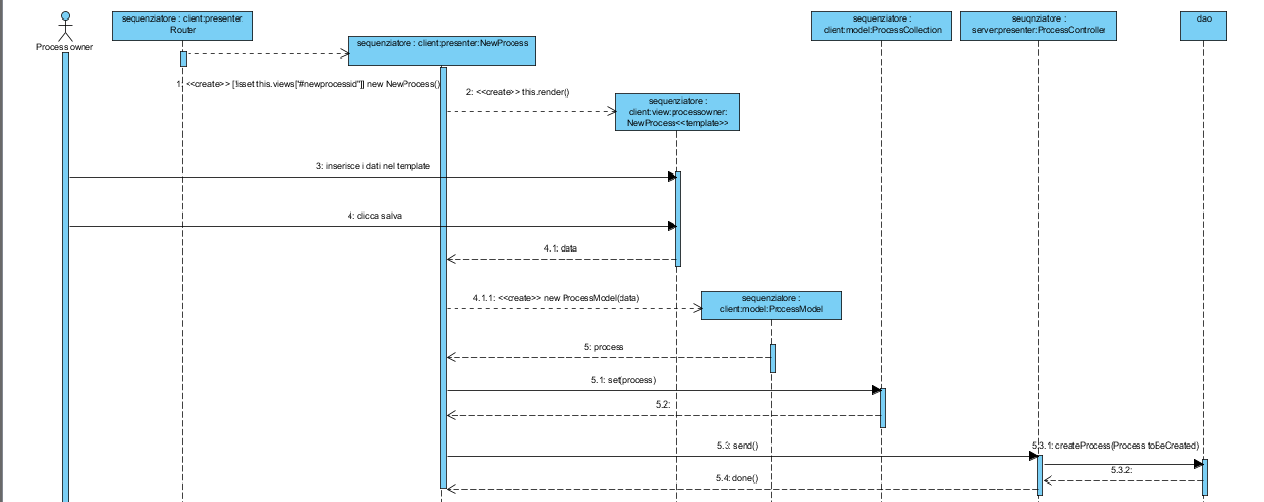
\includegraphics[scale=0.50]{./diagSequenza/creazioneprocesso.png}}
        \end{picture}
        \begin{center}
        Diagramma di sequenza - Creazione di un processo
        \end{center}
\paragraph{Descrizione della creazione di un processo}
La sequenza inizia con l'evento "creazione di un nuovo processo" da parte di un utente \textit{process owner}, quindi il client:presenter:router crea un oggetto di tipo client:presenter:NewProcess che a sua volta crea una view (tramite il relativo template) in modo che l'utente possa inserire i dati relativi al processo. Una volta che l'utente salva il processo, i dati vengono ritornati all'oggetto NewProcess, il quale crea un istanza (process) del client:model:ProcessModel; tramite il metodo \textit{set(process)} viene aggiornata la processCollection e viene inviata al server (messaggio sincrono send()) restando quindi in attesa del messaggio di conferma, da qui il server si occupa di "creare" effettivamente il suddetto processo (metodo \textit{createProcess(ProcessToBeCreated)}), ed una volta fatto, comunicherà al client l'avvenuta creazione, terminando la sequenza.
        
\subsection{Approvazione di un passo}
\setlength{\unitlength}{1mm}\begin{picture}(0,70)
                \put(0,0){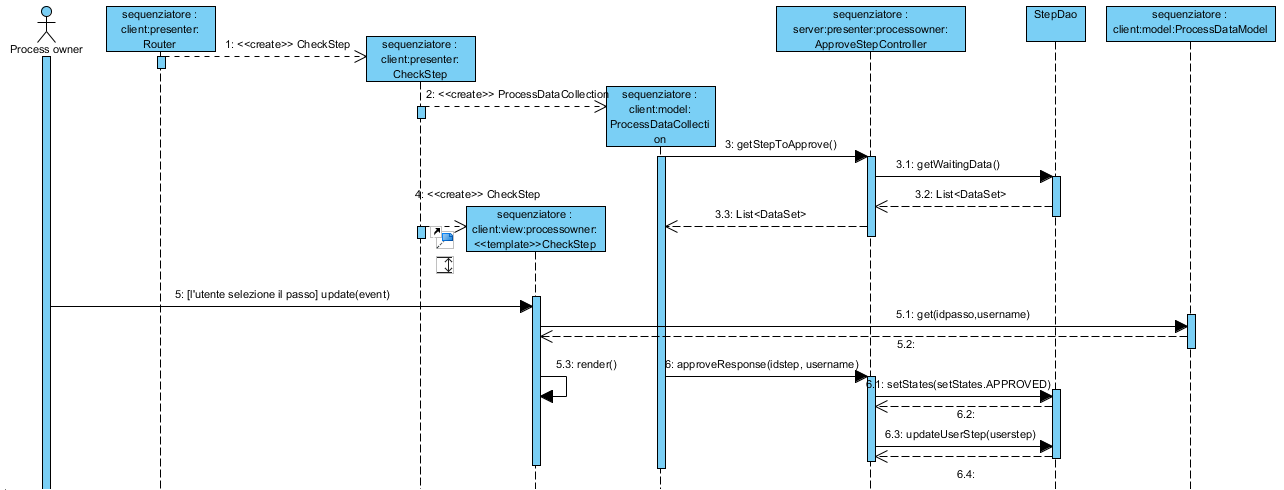
\includegraphics[scale=0.50]{./diagSequenza/approvazionepasso.png}}
        \end{picture}
         \begin{center}
        Diagramma di sequenza - Approvazione di un passo
        \end{center}
\paragraph{Descrizione dell'approvazione di un passo}
Il goal è quello di riuscire a confermare un passo in attesa di approvazione.
La sequenza inizia con il \textit{client:presenter:Router} che crea un nuovo oggetto \textit{client:presenter:CheckStep}, tale oggetto a sua volta crea un oggetto \textit{client:model:ProcessDataCollection} che richiede al server tramite il metodo \textit{getStepToApprove()} la lista di tutti i passi in attesa di conferma.
Lato server il \textit{presenter:processowner:ApproveStepController} viene istanziato, in seguito tale oggetto invia una richiesta (\textit{getWaitingData()}) allo StepDao e resta in attesa di ricevere i suddetti dati, ossia la lista dei passi in attesa di approvazione.
Una volta ottenuta tale lista, essa viene ritornata al client (più precisamente al model:ProcessDataCollection) traimte \textit{List<DataSet>}, altempo viene creata una view tramite la quale l'utente può scegliere il passo da approvare, una volta fatto, tramite il metodo \textit{approveResponse(idstep, username)} il client comunica al server il passo approvato, ed il server tramite \textit{setStates(setStates.APPROVED)} attua la reale modifica nello stepDao confermando il passo selezionato, terminando la sequenza.
        
\subsection{Registrazione}
\setlength{\unitlength}{1mm}\begin{picture}(0,70)
                \put(0,0){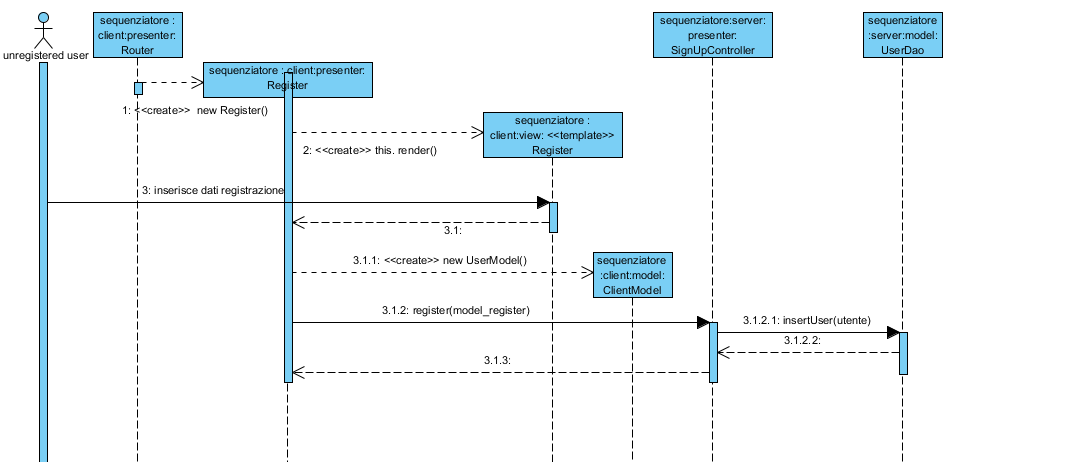
\includegraphics[scale=0.50]{./diagSequenza/sequenzaregistrazione.png}}
        \end{picture}
         \begin{center}
        Diagramma di sequenza - Registrazione di un utente
        \end{center}
\paragraph{Deacrizione della Registrazione utente}
In questo diagramma di attività viene mostrato lo scenario di registrazione di un nuovo utente.
La sequenza inizia sempre dal client:presenter:router che crea un oggetto della classe \textit{client:presenter:Register}, tramite il metodo \textit{render} si crea la view con cui l'utente può interagire inserendo i dati relativi alla sua registrazione. 
Raccolti i dati essi vengono ritornati al \textit{client:presenter:Register} il quale istanzia un nuovo oggetto (attraverso i costruttore:\textit{ new UserModel()}) di classe \textit{client:model:ClientModel } tale oggetto è poi utilizzato come parametro nel metodo \textit{register(model\_register)}. Quest'ultimo messaggio sincrono attende la risposta del server circa l'avvenuta inserzione del nuovo user nel database. Lato server quindi tramite il metodo \textit{insertUser(utente)} l'utente viene effettivamente registrato, e di conseguenza il server lo comunica al client, terminando la sequenza.